\chapter{关于全空间弹性波无相位数据成像算法的讨论} \label{rtm_phaseless}
在本章中, 我们基于逆时偏移算法, 针对全空间弹均匀弹性背景介质的障碍物成像问题测试一种新的直接成像法. 该算法仅利用弹性波总场在接收面法向和切向的模作为数据, 不需要障碍物的先验信息.在附录最后, 我们用大量数值算例来说明该算法的有效性.
\section{问题介绍}
假设 $D$ 是 $\R^2$ 中有界 Lipschitz 区域, $\nu_D$ 是其边界 $\Ga_D$ 上的外法向. 全空间背景介质与上文中半空间背景介质参数设置相同.假设在 $\pa B_s$ 和 $\pa B_r$ 上分别均匀分布着 $N_s$ 个弹性波发射器和 $N_r$ 个弹性波接收器, 其中 $\pa B_s$ 和 $\pa B_r$ 分别是圆心在原点,半径为 $R_s$ 和 $R_r$ 的圆 $B_s$ 和 $B_r$.定义 $\Om$ 是成像样本区域, 且有 $D\subset\Om\subset B_s, \  B_r$.假设入射场由位于 $\pa B_s$ 的点源 $x_s$ 沿着极化方向 $q$ 激发,记为 $u^i_q(x,x_s)=\G(x,x_s)q$.我们考虑障碍物满足刚体边界条件(Dirichlet 边界条件)情形,于是, 总场 $u_q(x,x_s)$ 满足以下方程:
\be
& &\Delta_e u_q(x,x_s)+ \omega^2u_q(x,x_s)= -\delta_{x_s}(x)\ \ \ \ \mbox{in }\ \ \ \R^2\bks \bar{D},\\ 
& &u_q(x,x_s)=0 \ \  \ \ \ \  \ \ \mbox{on} \ \Ga_D,\  \\
& & u_q(x,x_s) \ \ \ \ \ \ \mbox{满足 Kupradze's 辐射条件}. 
\ee
于是散射数据 $u^s_q(x,x_s)=u_q(x,x_s)-u^i_q(x,x_s)$.
\section{全空间弹性波无相位逆时偏移算法}
在文献 \cite{chen2015reverse_elas} 中, 通过在$\pa B_r$ 上的 $N_r$ 个接收器上测量的全相位数据 $u_q(x_r,x_s)$, 其中 $s=1,\cdots, N_s$, $r=1,\cdots, N_r$, 基于加权逆时偏移算法来对障碍物成像, 即有:
\ben
 I_{RTM
}(z)=-\om^2\Im\sum_{q=e_1,e_2}\frac{2\pi R_s}{N_s}\frac{2\pi R_r}{N_r}\sum_{s=1}^{N_s}\sum_{r=1}^{N_r}\bigg(c_p\G_p(z,x_rs)q+c_s\G_s(z,x_s)q\bigg)\\
\cdot\bigg(c_p\G_p(z,x_r)+c_s\G_s(z,x_r)\bigg)\overline{u^s_q(x_r,x_s)}ds(x_r)ds(x_s).
\een
$I_{RTM
}(z)$ 可以看做采用数值积分对如下连续函数的逼近,
\ben
\hat{I}_{RTM
}(z)=-\om^2\Im\sum_{q=e_1,e_2}\int_{\Ga_s}\int_{\Ga_r}\bigg(c_p\G_p(z,x_rs)q+c_s\G_s(z,x_s)q\bigg)\\
\cdot\bigg(c_p\G_p(z,x_r)+c_s\G_s(z,x_r)\bigg)\overline{u^s_q(x_r,x_s)}ds(x_r)ds(x_s).
\een
关于向量 $x=(x_1,x_2)^T$, 我们定义相应的径向单位向量 $\hat{x}={x}/{|x|}:=(\hat{x}_1,\hat{x}_2)^T$ 和周向单位向量 $\tilde{x}=(-\hat{x}_2,\hat{x}_1)$. 进一步, 定义二阶张量 $A(x)=\hat{x}\hat{x}^T$ 和 $B(x)=\tilde{x}\tilde{x}^T$.通过观察弹性波 $\G(x,y)$在无穷远处的渐近性质, 我们可以将成像函数 $\hat{I}_{RTM
}(z)$ 近似简化成只需要使用声波基本解 $g_k(x,y)$ 的成像函数 $\hat {I}_{RTM}^{lite}(z)$,
\ben
\hat {I}_{RTM}^{lite}(z)=-\Im\sum_{q=e_1,e_2}\int_{\Ga_s}\int_{\Ga_r}\bigg(k_pg_p(z,x_rs)A(x_s)q+k_sg_s(z,x_s)B(x_s)q\bigg)\\
\cdot\bigg(k_pg_p(z,x_r)A(x_r)+k_sg_s(z,x_r)B(x_r)\bigg)\overline{u^s_q(x_r,x_s)}ds(x_r)ds(x_s).
\een

\begin{lem}\label{kir_eq}
	对于任意 $|z|,|y|< R$, 成立
	\ben
	k_p\int_{|x|=R}g_p(z,x)A(x)\overline{\G(x,y)}ds(x)=\Im \G_p(z,y) +\W_p(y,z),\\
	k_s\int_{|x|=R}g_s(z,x)B(x)\overline{\G(x,y)}ds(x)=\Im \G_s(z,y) +\W_s(y,z),
	\een
	其中 $|\W_\alpha^{ij}(z,y)|+k_\alpha^{-1}|\nabla_z \W_\alpha^{ij}(z,y)|\leq C_\alpha R^{-1}$ 且常数 $C_\alpha$ 只依赖于 $k_\alpha|z|,k_\alpha|y|$, $\alpha\in\{p,s\}$.这里 $\W_\alpha^{ij}(z,y)$ 表示矩阵 $\W_s(y,z)$ 第 (i,j) 个元素.
\end{lem}
\debproof
首先, 我们回忆关于 Hankel 函数的估计 \cite[p.197]{watson1995treatise}, 对于任意 $t>0$, 我们有
\ben
& &H^{(1)}_0(t)=\left(\frac 2{\pi t}\right)^{1/2}e^{\i(t-\pi/4)}+R_0(t), \\
& &H^{(1)}_1(t)=\left(\frac 2{\pi t}\right)^{1/2}e^{\i(t-3\pi/4)}+R_1(t),
\een
这里存在与$t$无关的常数$C>0$, 成立 $|R_j(t)|\le Ct^{-3/2}$, $j=0,1$.于是, 利用弹性波基本解的表达式, 我们有
\ben
& &\G_p(x,y)=\frac{\i}{\sqrt{8\pi}(\lambda+2\mu)}A(x-y)\frac{1}{(k_p|x-y|)^{1/2}}e^{\i k_p|x-y|-\i\frac{\pi}{4}}+O(\frac{1}{(k_p|x-y|)^{3/2}}),\\
& &\G_s(x,y)=\frac{\i}{\sqrt{8\pi}\mu}B(x-y)\frac{1}{(k_s|x-y|)^{1/2}}e^{\i k_p|x-y|-\i\frac{\pi}{4}}+O(\frac{1}{(k_s|x-y|)^{3/2}}).
\een
通过简单的计算, 可得
\ben 
|A(x-y)-A(x)|\leq C_1/|x|, \ \ |B(x-y)-B(x)|\leq C_2/|x| ,\\
\left|\frac{1}{|x-y|}-\frac{1}{|x|}\right|\leq C_3/|x|^2 , \ \
||x-y|-(|x|-\hat{x}\cdot y)|\leq C_4/|x|,
\een
这里常数 $C_i>0$, i=1,2,3,4 且仅依赖于 $|y|$. 于是, 我们有
\ben
& &\G_p(x,y)=\frac{\i}{\sqrt{8\pi}(\lambda+2\mu)}A(x)\frac{1}{(k_p|x|)^{1/2}}e^{\i k_p(|x|-\hat{x}\cdot y)-\i\frac{\pi}{4}}+\gamma_p(x,y),\\ 
& &\G_s(x,y)=\frac{\i}{\sqrt{8\pi}\mu}B(x)\frac{1}{(k_s|x|)^{1/2}}e^{\i k_s(|x|-\hat{x}\cdot y)-\i\frac{\pi}{4}}+\gamma_s(x,y), \\
& &g_\alpha(x,y)=\frac{\i}{\sqrt{8\pi}}\frac{1}{(k_\alpha|x|)^{1/2}}e^{\i k_s(|x|-\hat{x}\cdot y)-\i\frac{\pi}{4}}+\gamma(x,y),\ \ \ \al=p,s \ ,
\een
其中 $|\gamma_\alpha(x,y)|\leq C(k_\alpha|x|)^{-3/2}$ , $\alpha\in\{p,s\}$且常数 $C>0$ 仅依赖于 $k_\alpha|y|$.将上述估计代入积分式,引理得证.
\finproof
通过引理 \ref{kir_eq} 和文献 \cite[定理 3.1]{ela_reverse}中的论证方法, 可得
\ben
|\hat{I}_{RTM
}(z)-\hat{I}_{RTM
}^{lite}(z)|\leq C\|T\|((k_p R_s)^{-1}+(k_p R_r)^{-1}),
\een
其中 $\|T\|$ 是散射问题的解算子的范数,常数 $C>0$ 与$D$, $k_p$, $k_s$ 无关.
 
上述成像算法需要散射场的全部相位信息,下面我们将只根据总场数据的振幅数据来成像.假设我们在接收面 $\pa B_r$ 上只能接收到法向 $\hat x_r$ 上和切向 $\tilde x_r$ 上的数据的模长,即 $|\hat{x_r}^Tu_q(x_r,x_s)|$ 和 $|\hat{x_r}^Tu_q(x_r,x_s)|$,于是我们提出针对该接收数据的直接成像法为:
\ben
\hat {I}_{RTM}^{phaseless}(z)=-\Im\sum_{q=e_1,e_2}\int_{\Ga_s}\int_{\Ga_r}\bigg(k_pg_p(z,x_rs)A(x_s)q+k_sg_s(z,x_s)B(x_s)q\bigg)\\
\cdot\bigg(k_pg_p(z,x_r)\hat{x_r}D_p(x_r,x_s)+k_sg_s(z,x_r)\tilde{x_r}D_s(x_r,x_s)\bigg)ds(x_r)ds(x_s),
\een
这里
\ben
D_p(x_r,x_s)=\frac{|\hat{x_r}^Tu_q(x_r,x_s)|^2-|\hat{x_r}^Tu^i_q(x_r,x_s))|^2}{\hat{x_r}^Tu^i_q(x_r,x_s))}, \\
D_s(x_r,x_s)=\frac{|\tilde{x_r}^Tu_q(x_r,x_s)|^2-|\tilde{x_r}^Tu^i_q(x_r,x_s))|^2}{\tilde{x_r}^Tu^i_q(x_r,x_s))}.
\een
利用 $|x|^2=x\hat x, \ \  x\in \C$, 我们可以得到,
\ben
D_p(x_r,x_s)&=&\hat{x_r}^T\overline{u^s_q}+\frac{|\hat{x_r}^Tu^s_q(x_r,x_s)|^2}{\hat{x_r}^Tu^i_q(x_r,x_s))}+\frac{(\hat{x_r}^Tu^s_q(x_r,x_s))(\hat{x_r}^T\overline{u^i_q(x_r,x_s)})}{\hat{x_r}^Tu^i_q(x_r,x_s))}  \\ 
&:=&\hat{x_r}^T\overline{u^s_q}+\Delta_p(x_r,x_s),\\
D_s(x_r,x_s)&=&\tilde{x_r}^T\overline{u^s_q}+\frac{|\tilde{x_r}^Tu^s_q(x_r,x_s)|^2}{\tilde{x_r}^Tu^i_q(x_r,x_s))}+\frac{(\tilde{x_r}^Tu^s_q(x_r,x_s))(\tilde{x_r}^T\overline{u^i_q(x_r,x_s)})}{\tilde{x_r}^Tu^i_q(x_r,x_s))} \\ 
&:=&\tilde{x_r}^T\overline{u^s_q}+\Delta_s(x_r,x_s).
\een

\begin{figure}
	\centering
	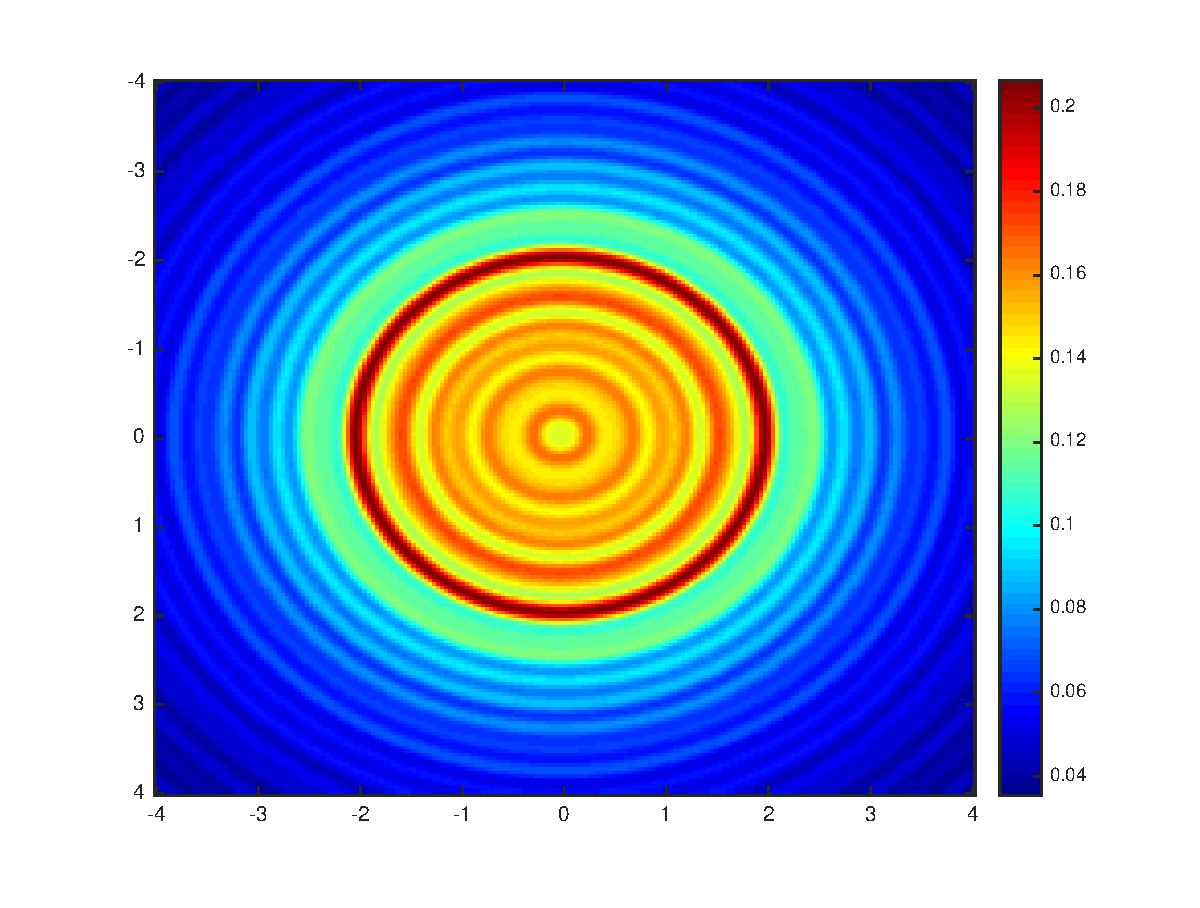
\includegraphics[width=0.28\textwidth]{./Img/graphic_phase/circle_r_10_k_4_vector.eps}
	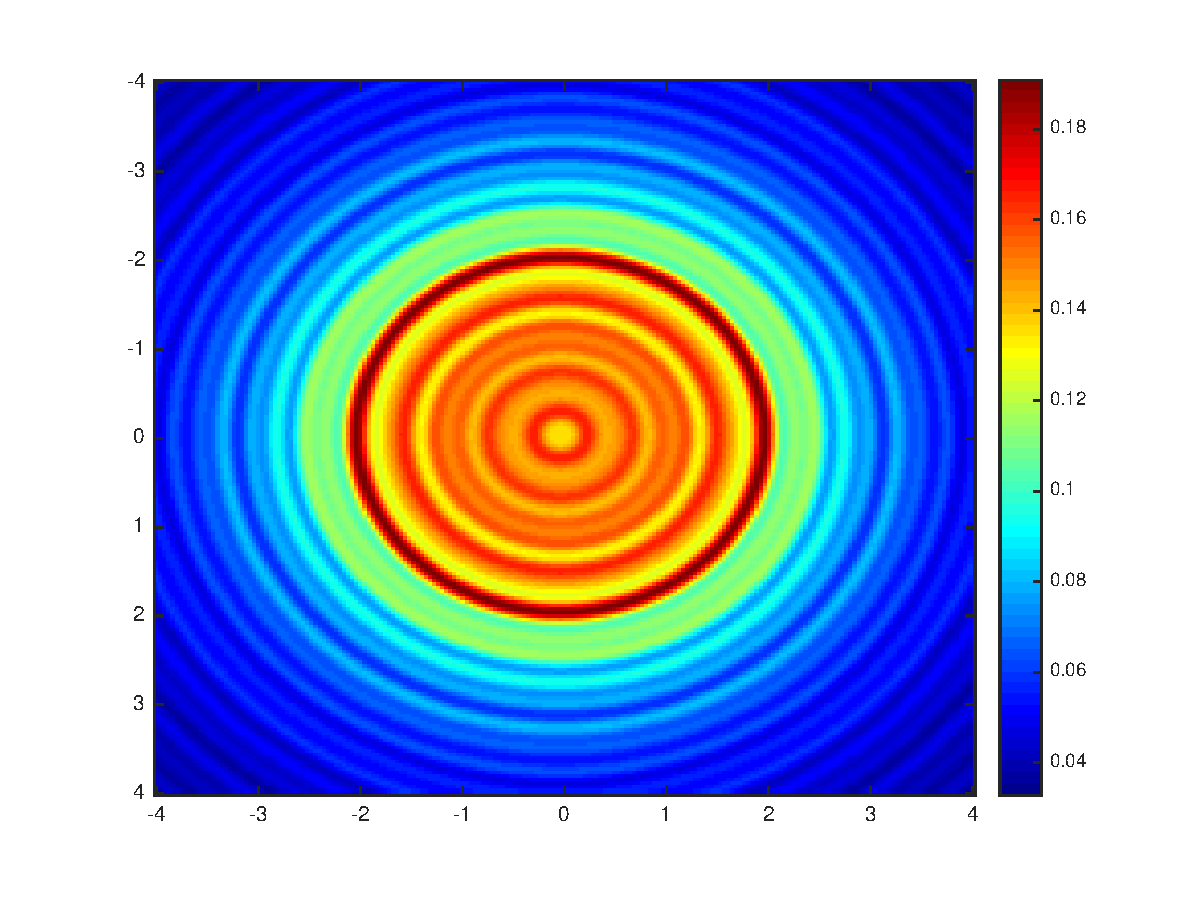
\includegraphics[width=0.28\textwidth]{./Img/graphic_phase/circle_r_10_k_4_scalar.eps}
	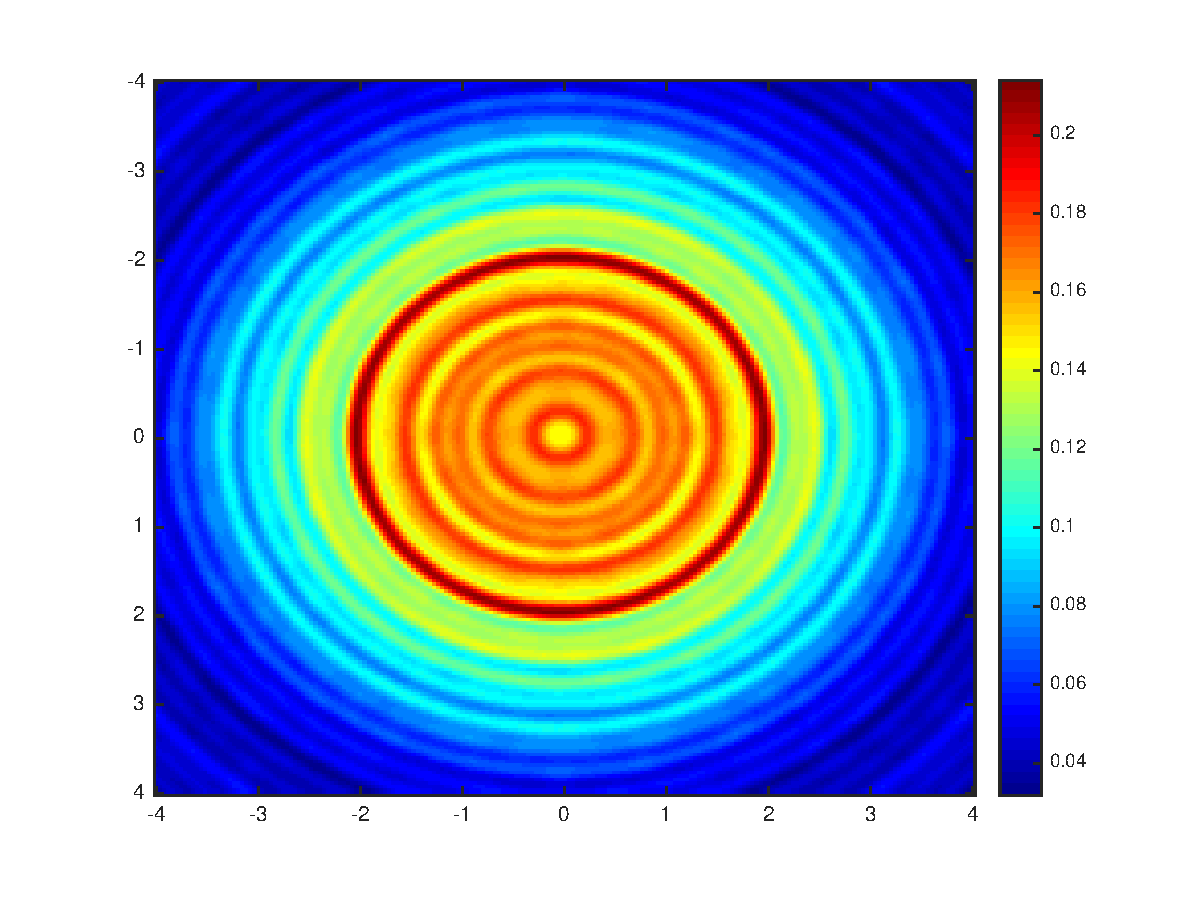
\includegraphics[width=0.28\textwidth]{./Img/graphic_phase/circle_r_10_k_4_phaseless_n_512_bias_100.eps}
	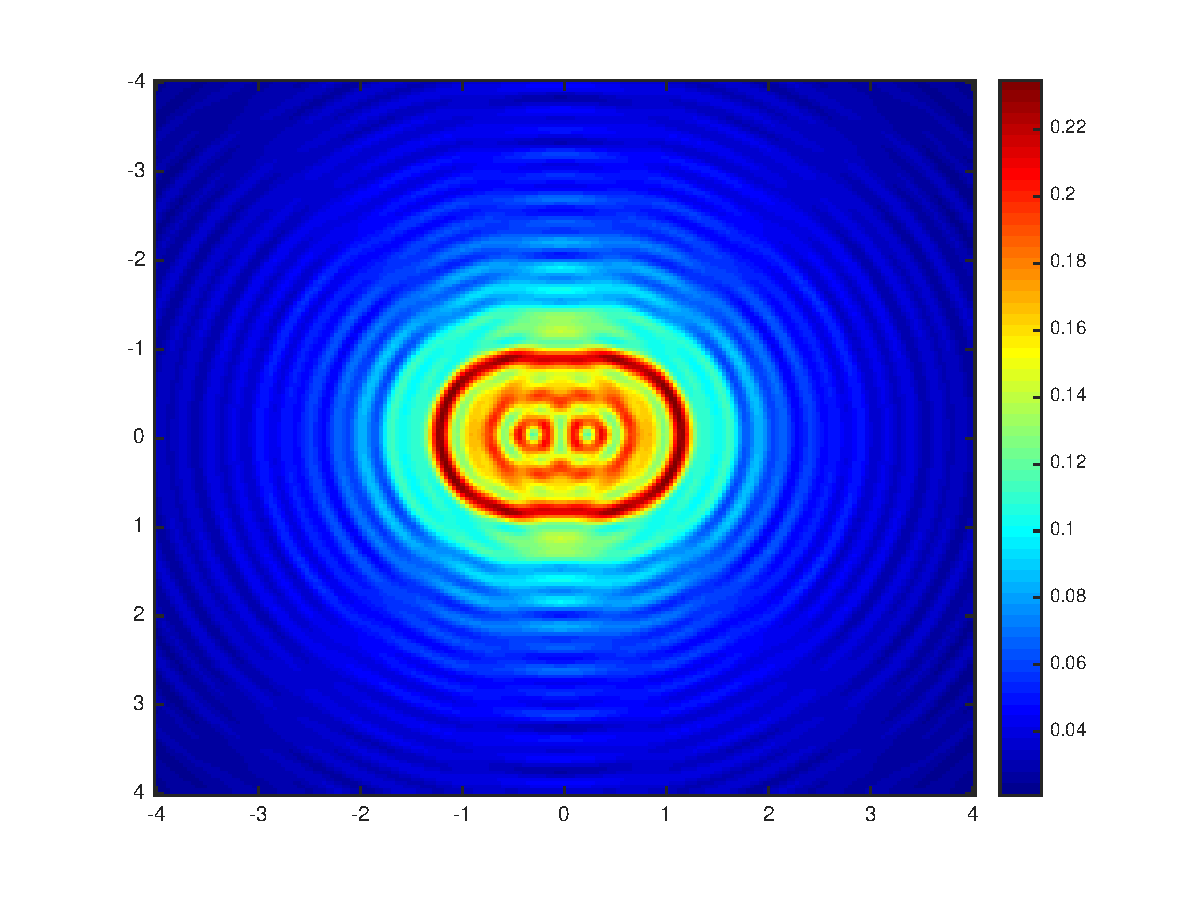
\includegraphics[width=0.28\textwidth]{./Img/graphic_phase/peanut_r_10_k_4_vector.eps}
	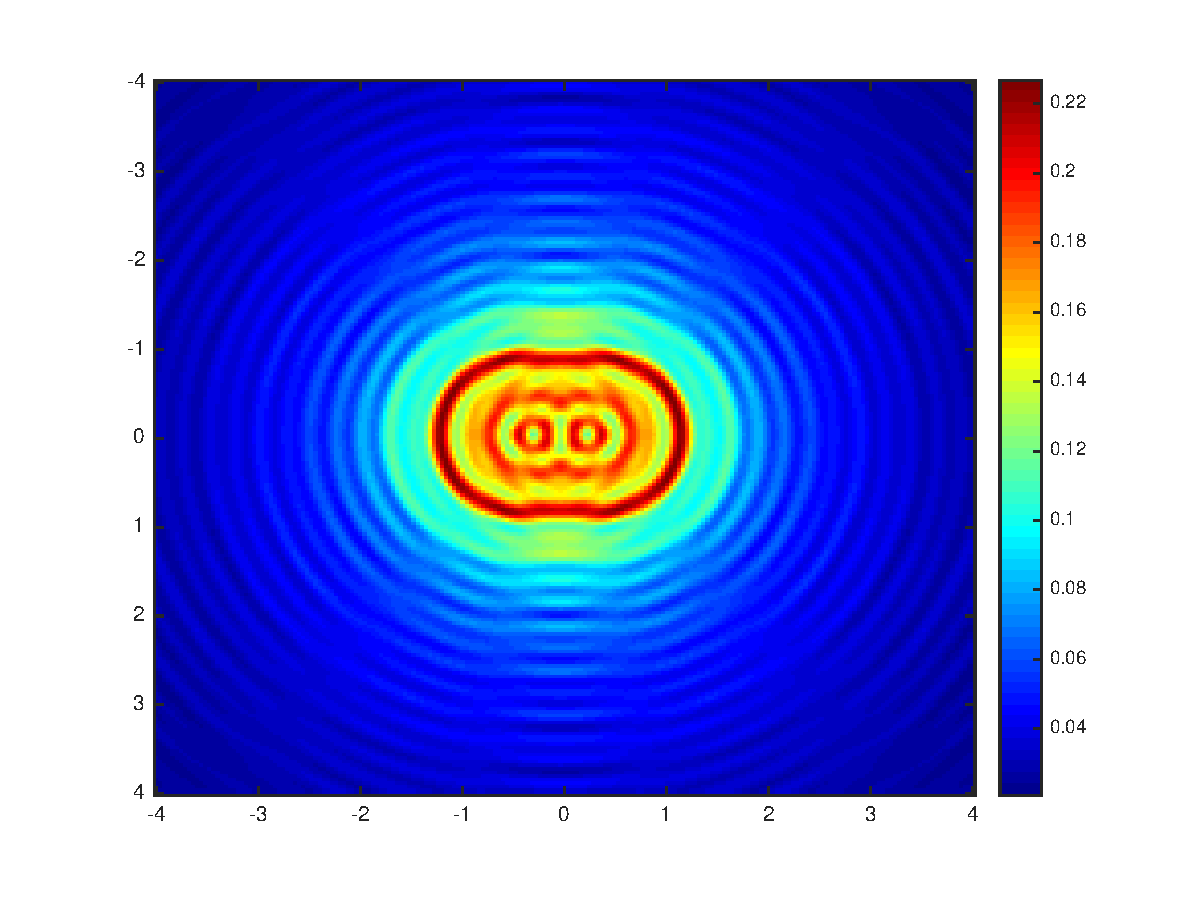
\includegraphics[width=0.28\textwidth]{./Img/graphic_phase/peanut_r_10_k_4_scalar.eps}
	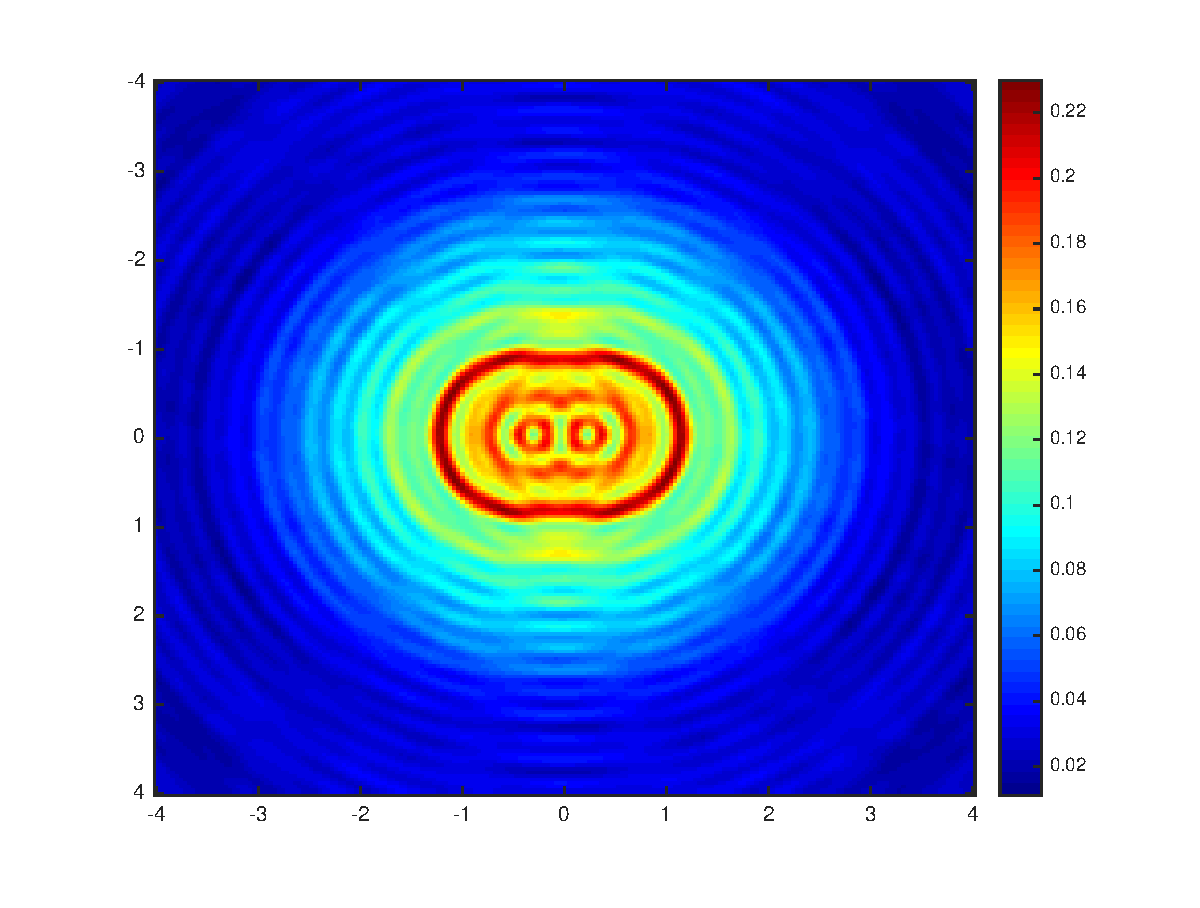
\includegraphics[width=0.28\textwidth]{./Img/graphic_phase/peanut_r_10_k_4_phaseless_n_512_bias_100.eps}
	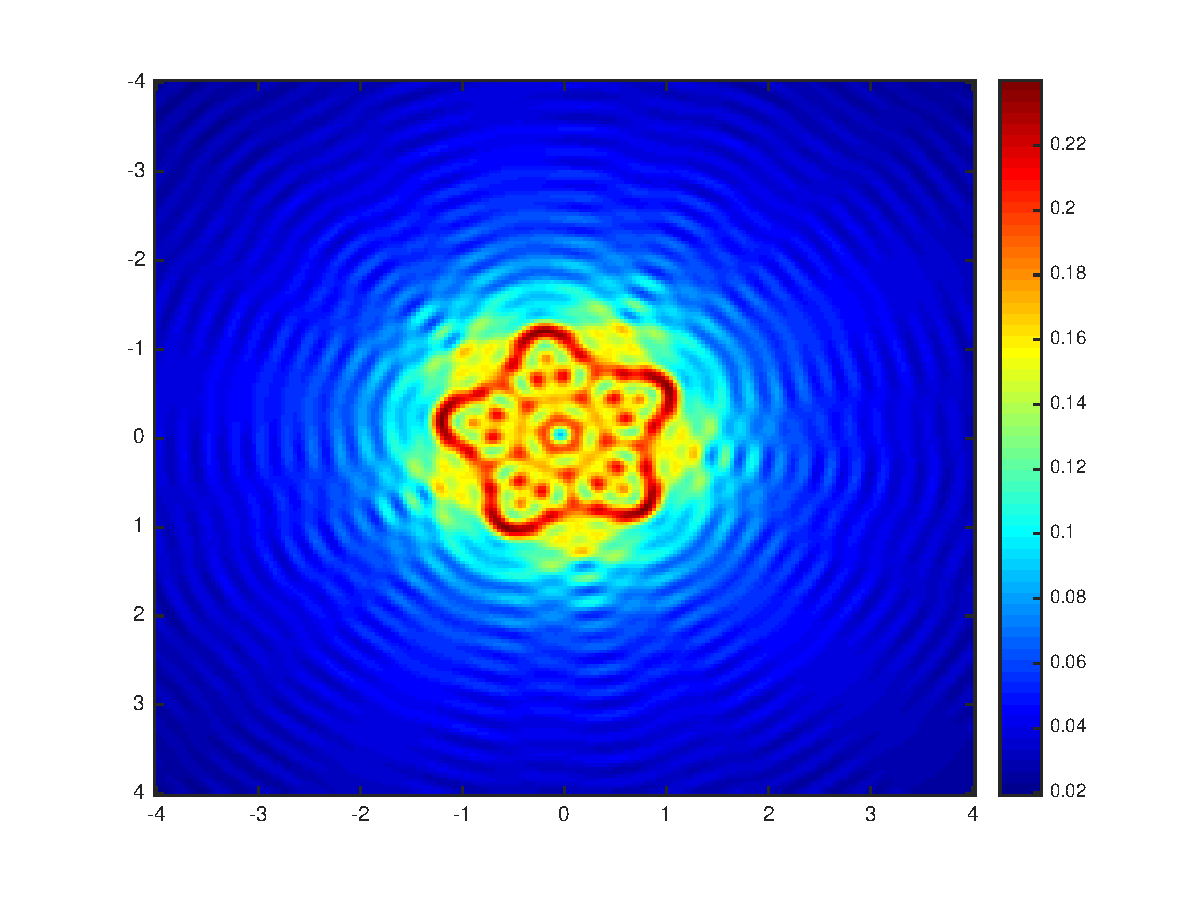
\includegraphics[width=0.28\textwidth]{./Img/graphic_phase/5-leaf_r_10_k_4_vector.eps}
	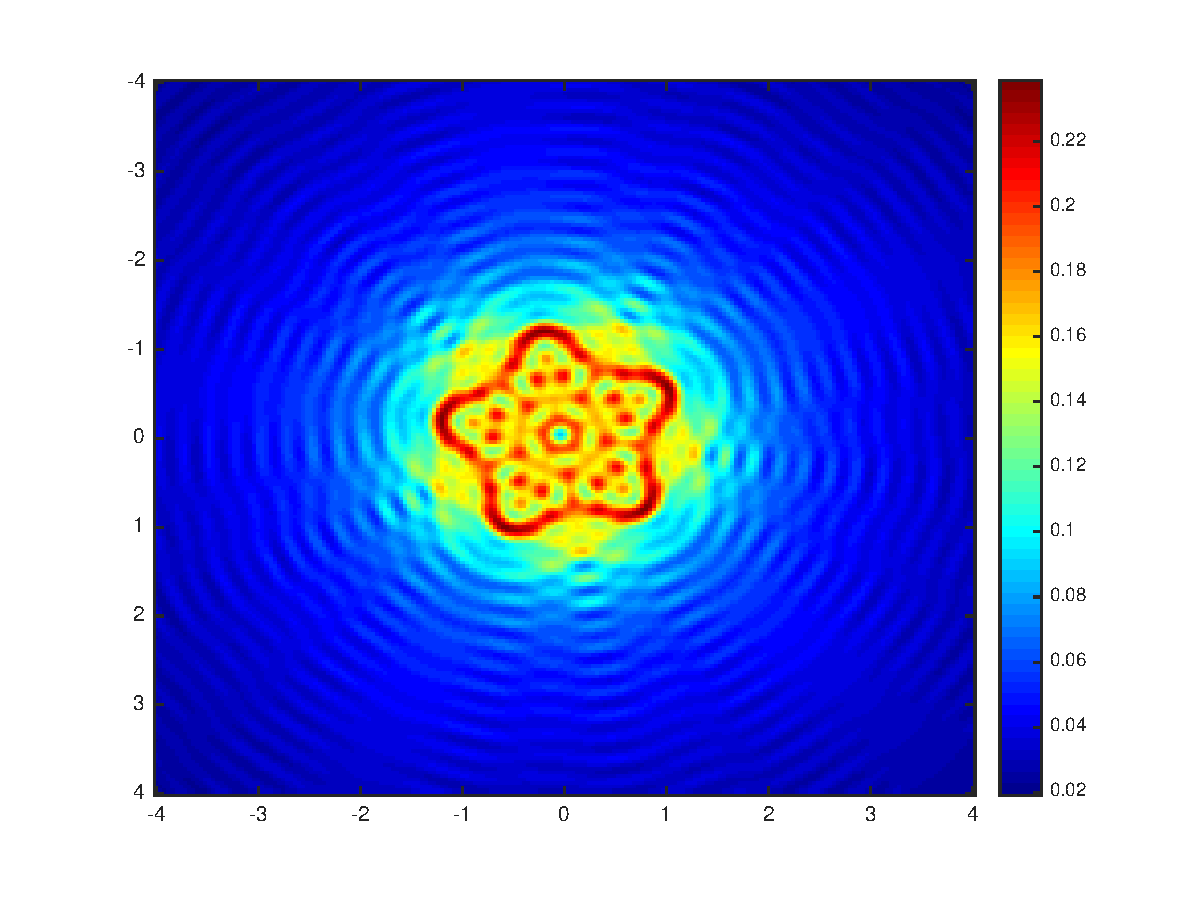
\includegraphics[width=0.28\textwidth]{./Img/graphic_phase/5-leaf_r_10_k_4_scalar.eps}
	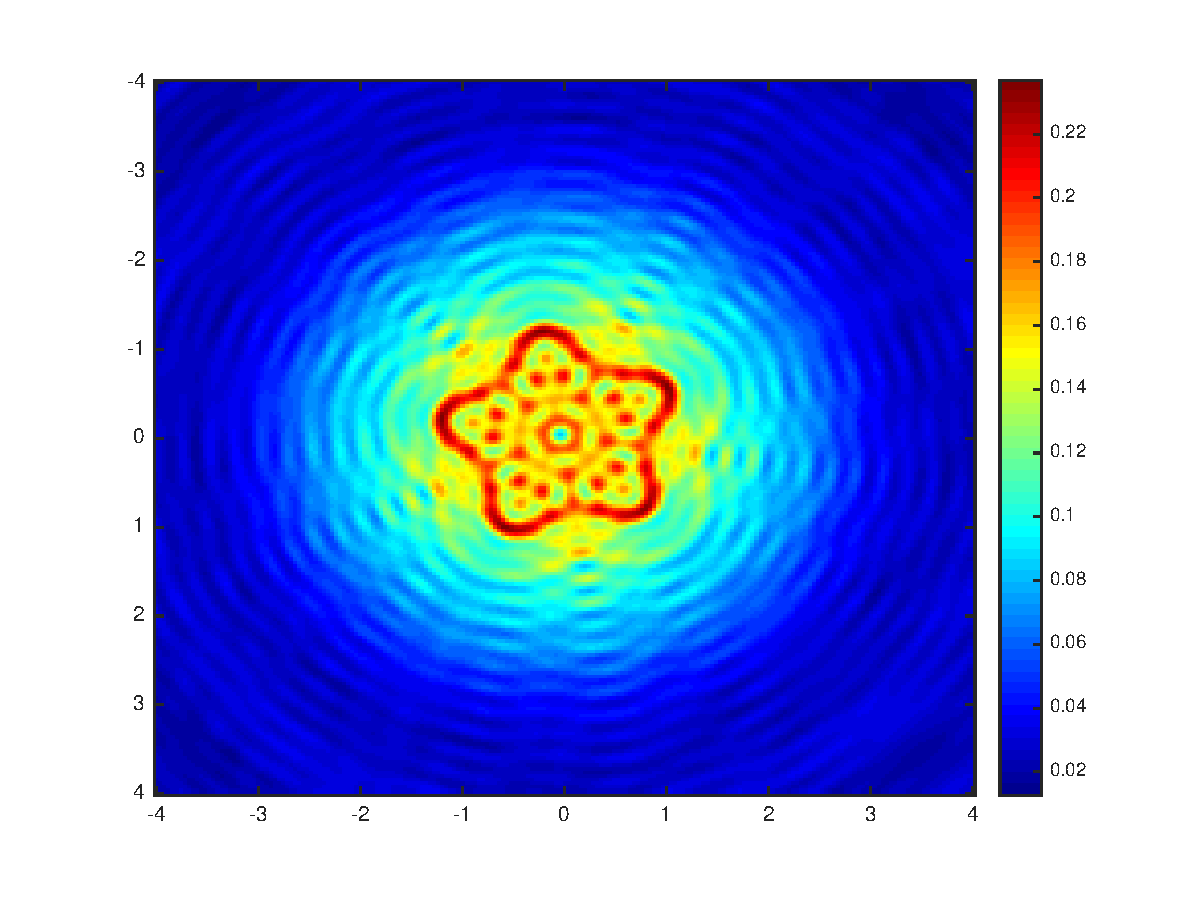
\includegraphics[width=0.28\textwidth]{./Img/graphic_phase/5-leaf_r_10_k_4_phaseless_n_512_bias_100.eps}
	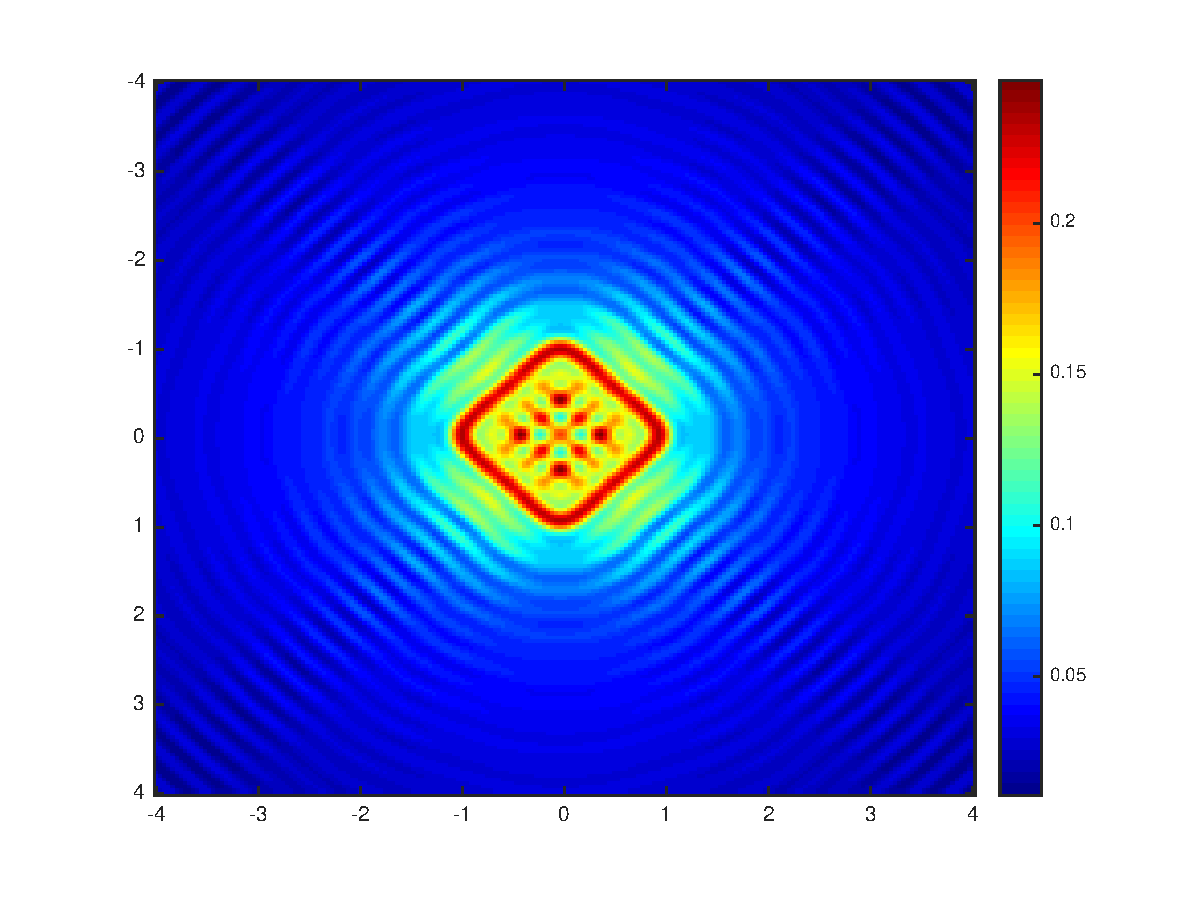
\includegraphics[width=0.28\textwidth]{./Img/graphic_phase/rectangle_r_10_k_4_vector.eps}
	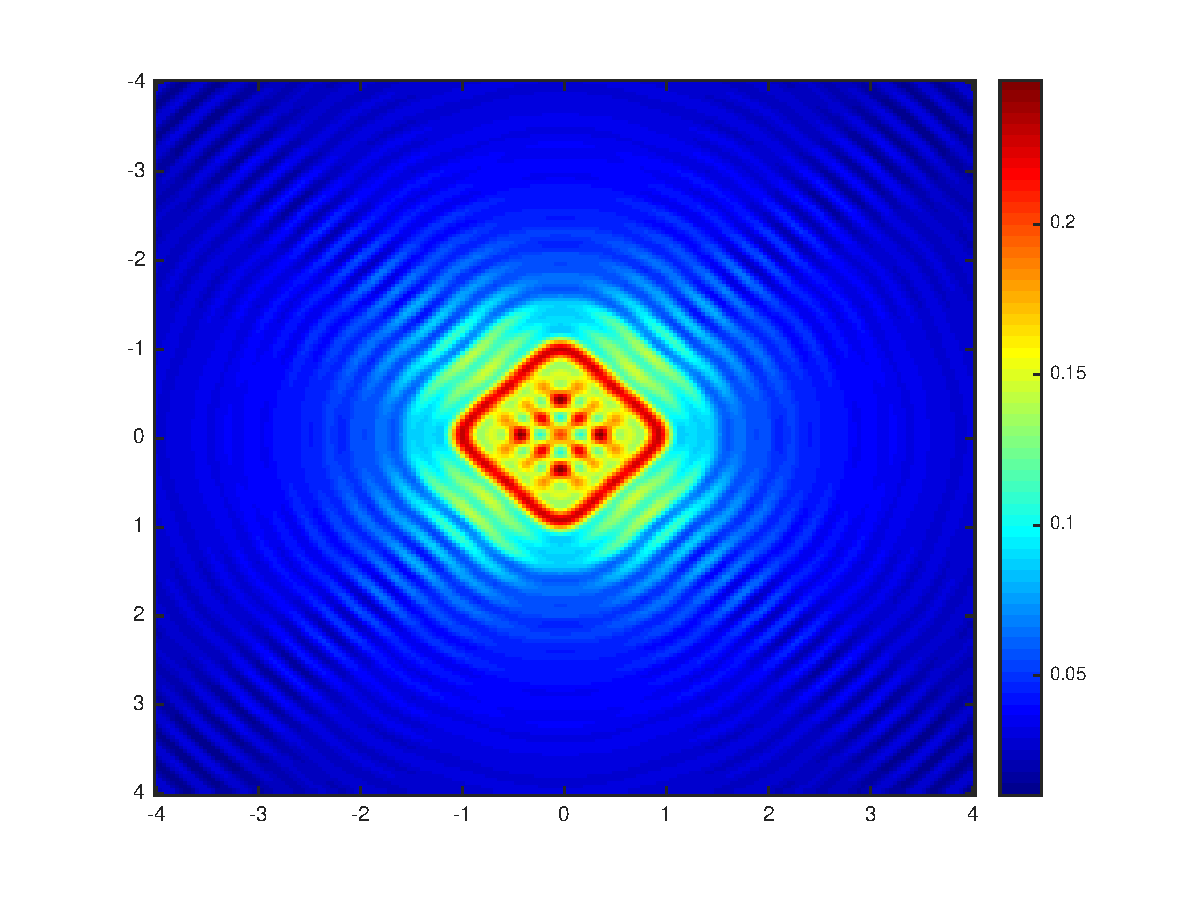
\includegraphics[width=0.28\textwidth]{./Img/graphic_phase/rectangle_r_10_k_4_scalar.eps}
	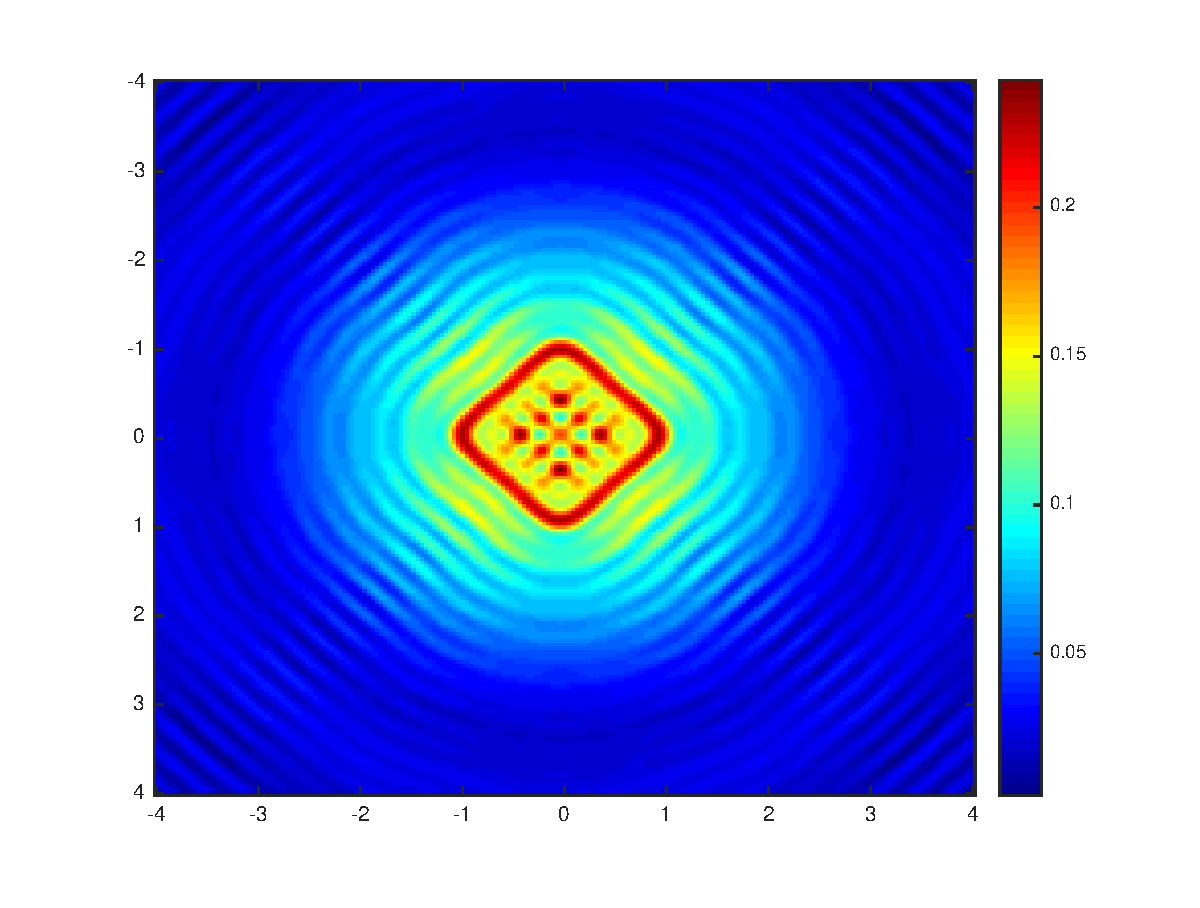
\includegraphics[width=0.28\textwidth]{./Img/graphic_phase/rectangle_r_10_k_4_phaseless_n_512_bias_100.eps}
	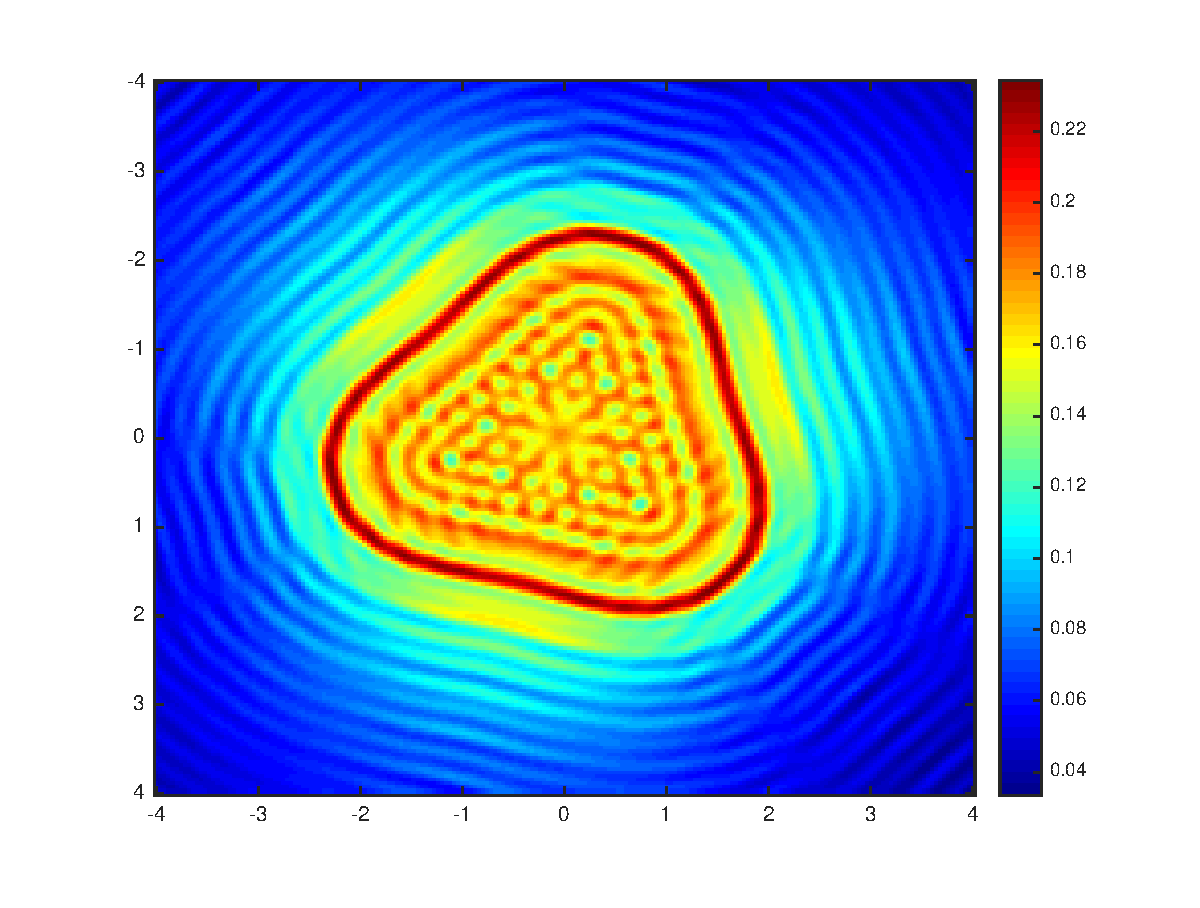
\includegraphics[width=0.28\textwidth]{./Img/graphic_phase/pear_r_10_k_4_vector.eps}
	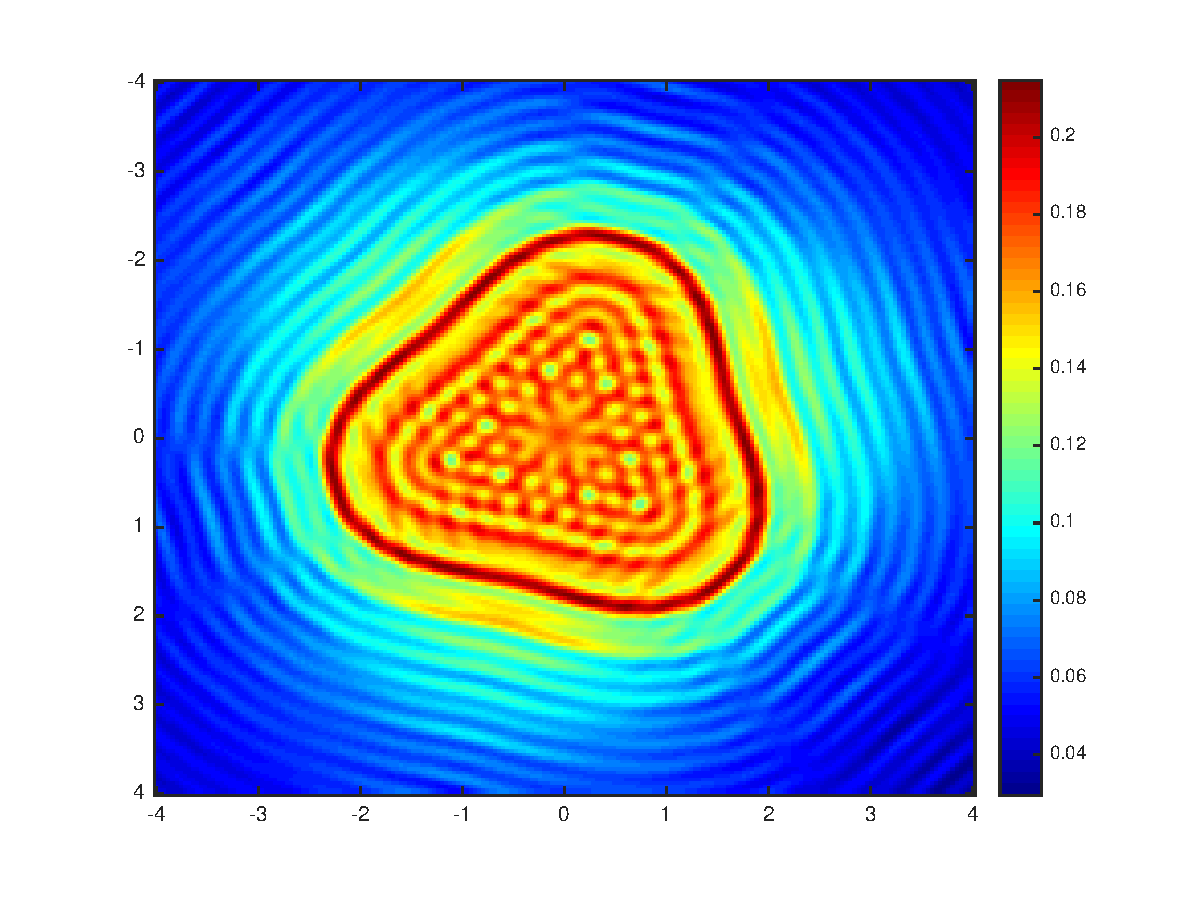
\includegraphics[width=0.28\textwidth]{./Img/graphic_phase/pear_r_10_k_4_scalar.eps}
	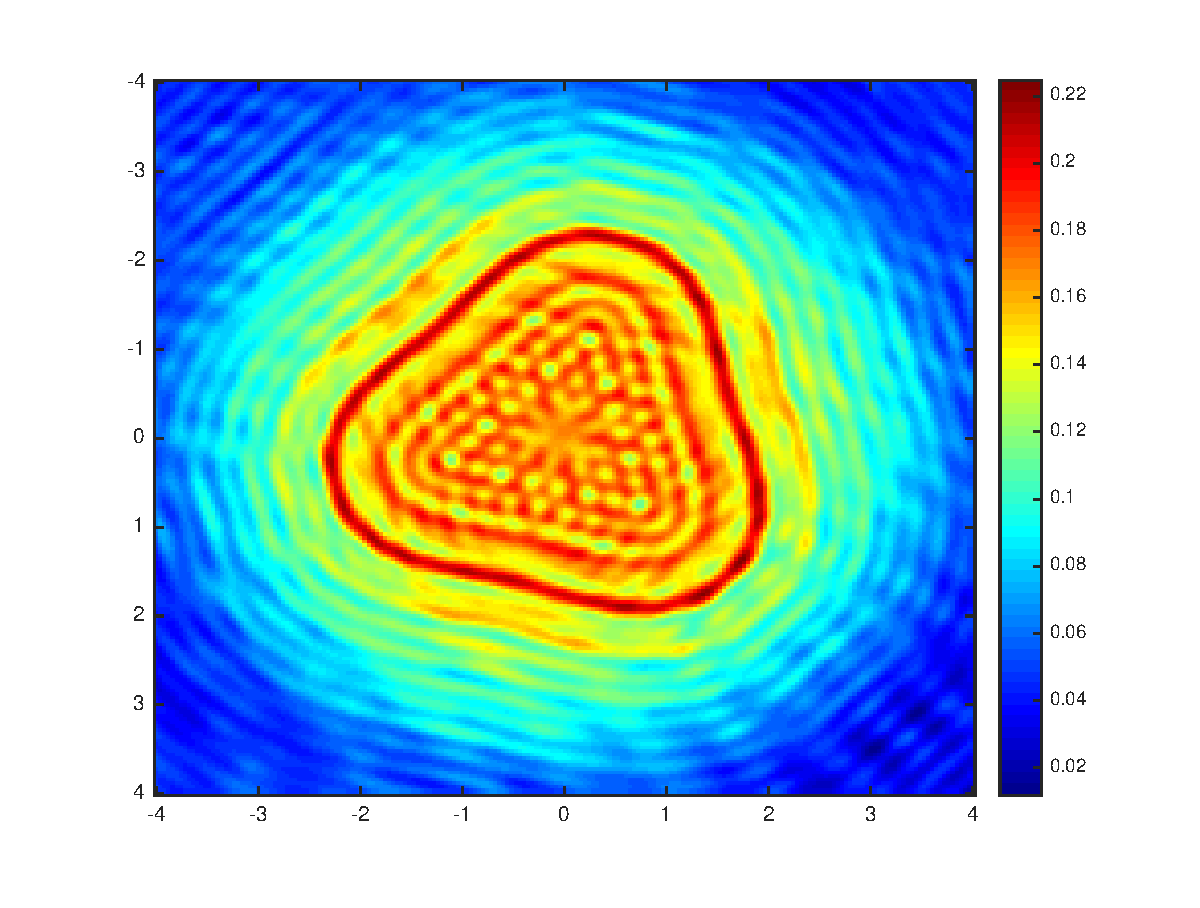
\includegraphics[width=0.28\textwidth]{./Img/graphic_phase/pear_r_10_k_4_phaseless_n_512_bias_100.eps}
	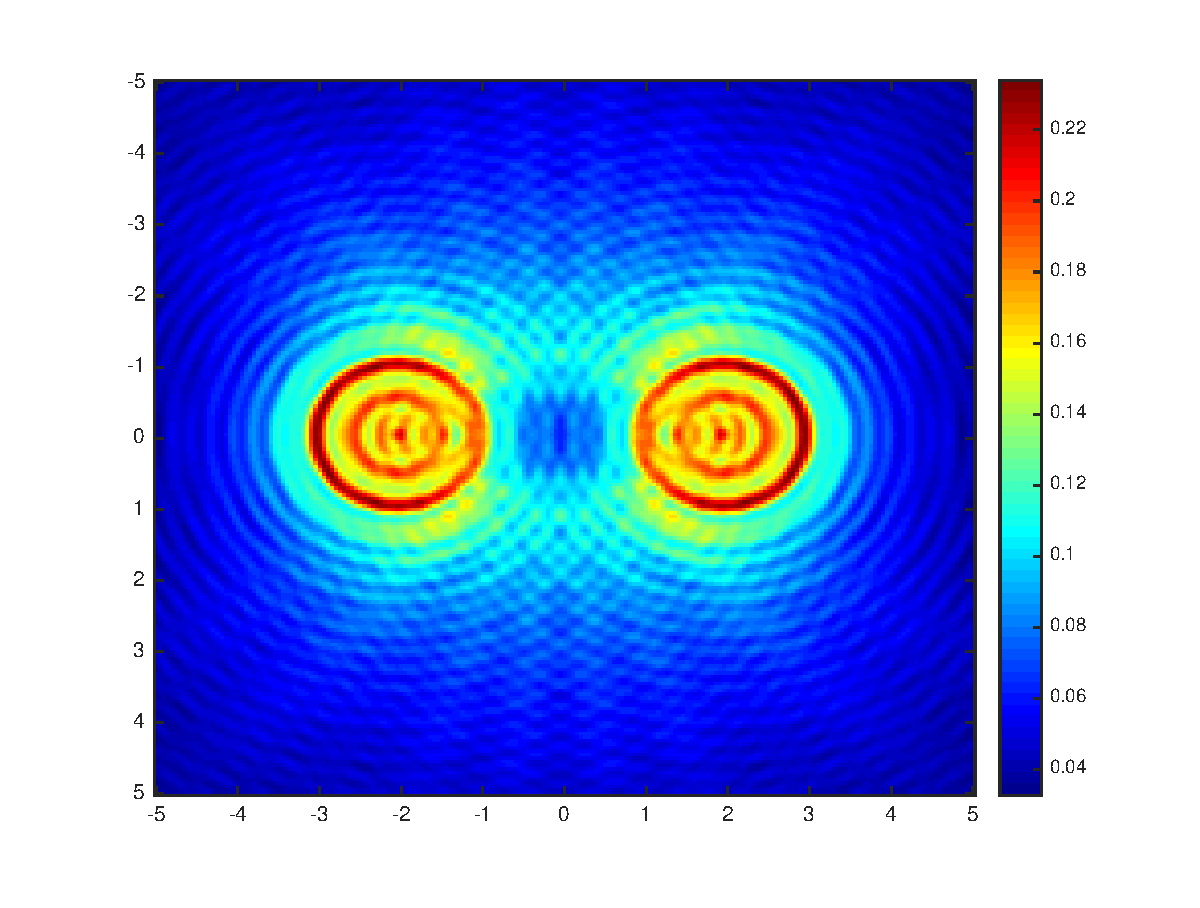
\includegraphics[width=0.28\textwidth]{./Img/graphic_phase/bi_circle_r_10_k_4_vector.eps}
	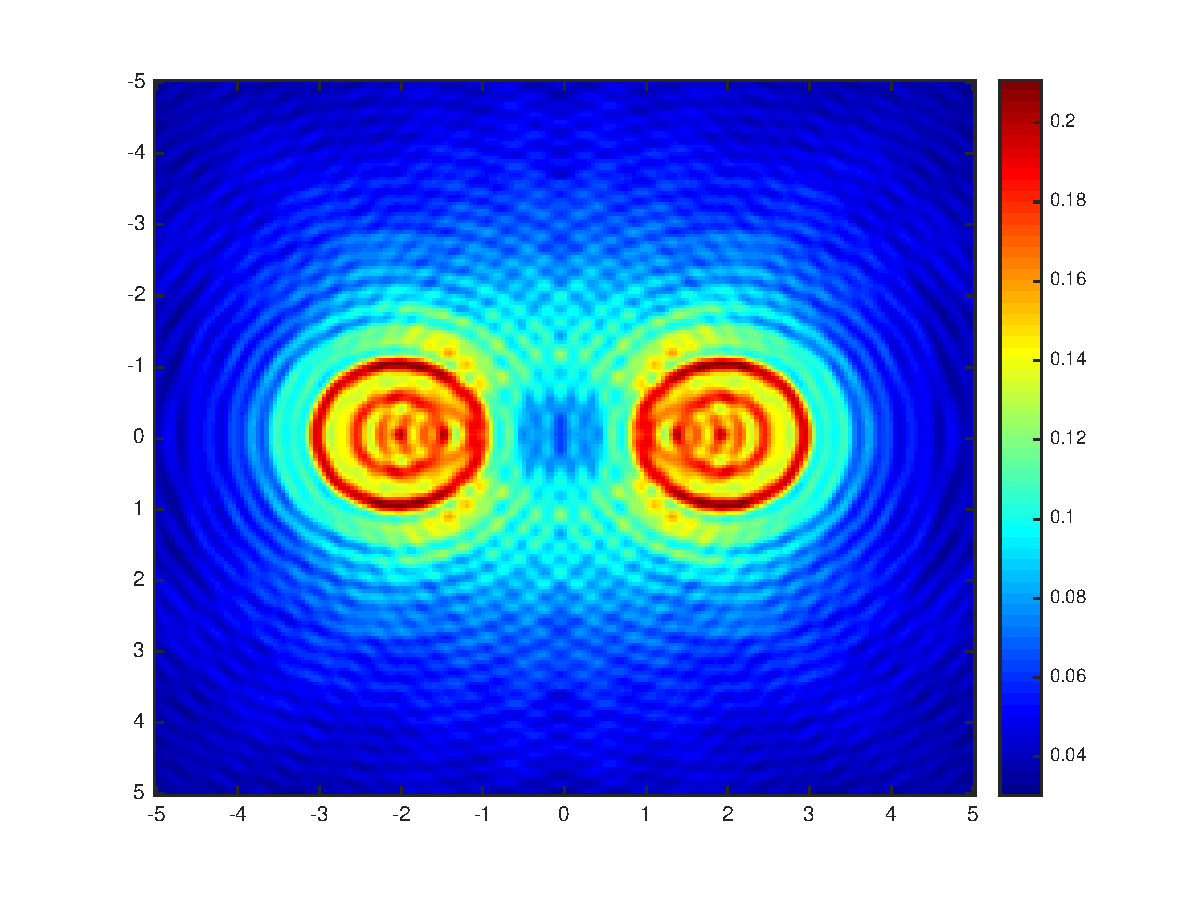
\includegraphics[width=0.28\textwidth]{./Img/graphic_phase/bi_circle_r_10_k_4_scalar.eps}
	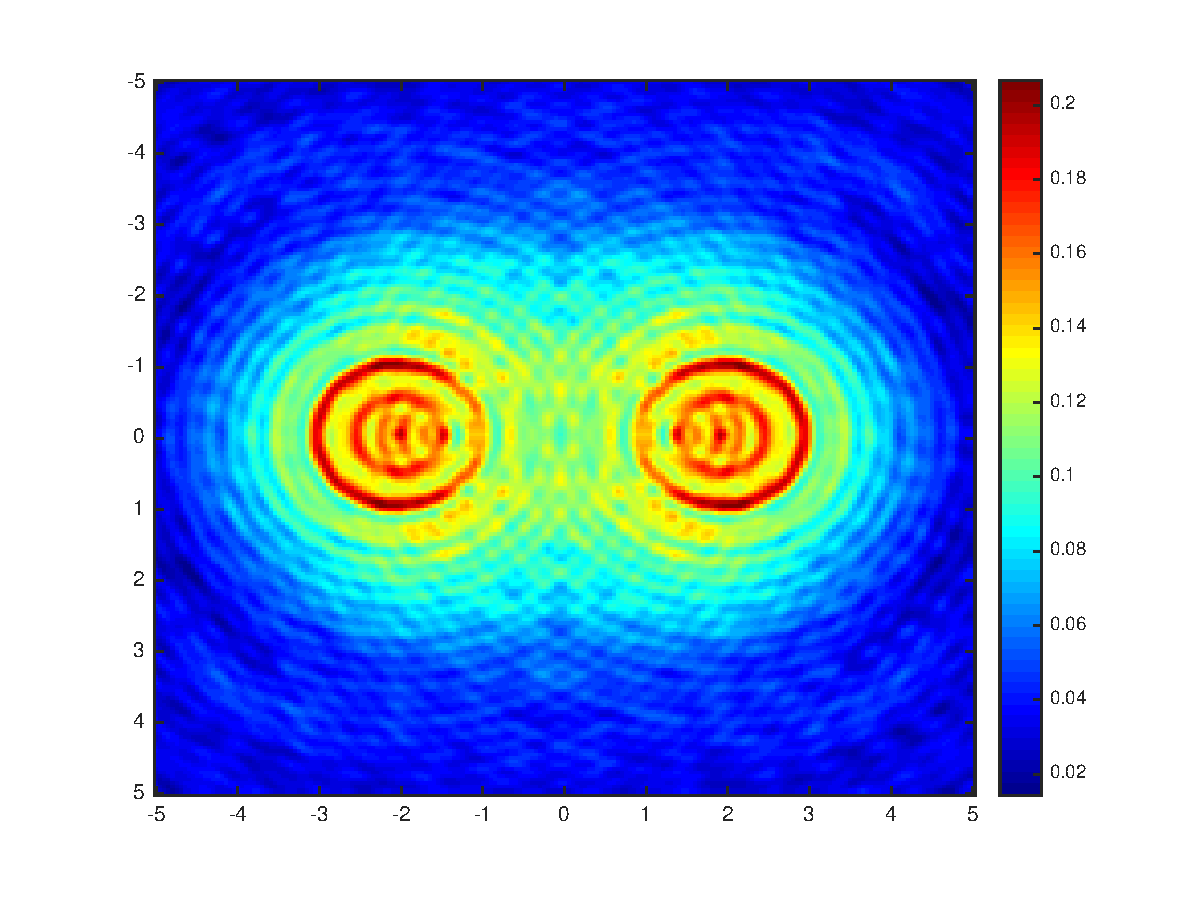
\includegraphics[width=0.28\textwidth]{./Img/graphic_phase/bi_circle_r_10_k_4_phaseless_n_512_bias_100.eps}
	\caption{所有测试中的样本区域都为:$[-4,4]\times[-4,4]$, 参数设置为:$\lambda=\mu=1,\om=4\pi,R_s=R_r=10$.不同行对应的是不同障碍物形状的测试,从左到右用到的成像函数分别是 $\hat{I}_{RTM}$, $\hat{I}_{RTM}^{lite}$, $\hat{I}_{RTM}^{phaseless}$. }\label{figure_phaseless}
\end{figure}


因此将上式代入 ${I}_{RTM}^{phaseless}(z)$,我们有 
\ben
\hat {I}_{RTM}^{phaseless}(z)&=&{I}_{RTM}^{lite}(z)-\Im\sum_{q=e_1,e_2}\int_{\Ga_s}\int_{\Ga_r}\bigg(k_pg_p(z,x_rs)A(x_s)q+k_sg_s(z,x_s)B(x_s)q\bigg)
\\ 
& &
\cdot\bigg(k_pg_p(z,x_r)\hat{x_r}\Delta_p(x_r,x_s)+k_sg_s(z,x_r)\tilde{x_r}\Delta_s(x_r,x_s)\bigg)ds(x_r)ds(x_s) \\
&:=&{I}_{RTM}^{lite}(z)+R(z).
\een
如下图\ref{figure_phaseless}所示, 无相位成像函数是有效的. 在理论分析方面, 我们将进一步研究 $|R(z)|$ 与 $R_s, R_r$ 的关系.


